\documentclass[tikz,border=4pt]{standalone}
\usepackage{tikz}

\begin{document}
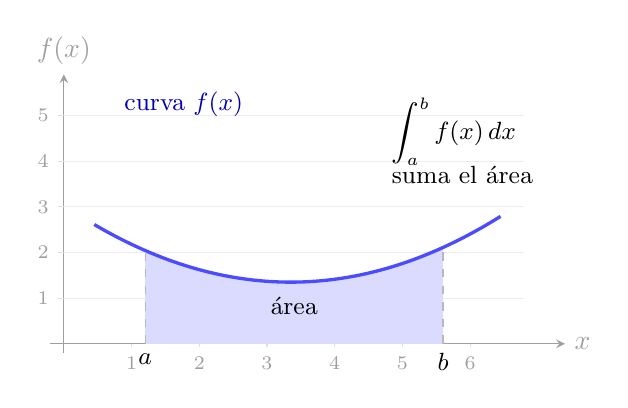
\begin{tikzpicture}[x=0.86cm,y=0.58cm,>=stealth]
  \draw[->,gray!75] (-0.2,0) -- (7.4,0) node[right] {$x$};
  \draw[->,gray!75] (0,-0.2) -- (0,5.9) node[above] {$f(x)$};

  \foreach \x in {1,2,3,4,5,6} {
    \draw[gray!25] (\x,0) -- (\x,-0.08) node[below,gray!75] {\scriptsize \x};
  }
  \foreach \y in {1,2,3,4,5} {
    \draw[gray!14] (0,\y) -- (6.8,\y);
    \draw[gray!25] (0,\y) -- (-0.08,\y) node[left,gray!75] {\scriptsize \y};
  }

  \fill[blue!14]
    (1.2,0) --
    plot[domain=1.2:5.6,samples=90,smooth] ({\x},{0.15*(\x-3.35)*(\x-3.35)+1.35}) --
    (5.6,0) -- cycle;

  \draw[domain=0.45:6.45,samples=100,smooth,very thick,blue!70]
    plot ({\x},{0.15*(\x-3.35)*(\x-3.35)+1.35});

  \draw[dashed,gray!55] (1.2,0) node[below,black] {\small $a$} -- (1.2,2.04);
  \draw[dashed,gray!55] (5.6,0) node[below,black] {\small $b$} -- (5.6,2.11);

  \node[anchor=west,blue!70!black] at (0.75,5.25) {\small curva $f(x)$};
  \node[align=center,black] at (3.4,0.82) {\small \'{a}rea};
  \node[anchor=west,align=left,black] at (4.7,4.45)
    {\small $\displaystyle \int_a^b f(x)\,dx$\\[-1pt]\small suma el \'{a}rea};
\end{tikzpicture}
\end{document}
